\documentclass[a4paper,11pt]{article}

\usepackage[plain]{fullpage} %Error.
\usepackage{graphicx}  %This enables the inclusion of pdf graphic files in figures
\usepackage{wrapfig}
\usepackage{array}
\usepackage[hidelinks]{hyperref}
\usepackage{color}
\definecolor{light-gray}{gray}{0.95}
\usepackage{listings}
\lstset{
basicstyle=\footnotesize, 
morecomment=[l]{/*},
backgroundcolor=\color{light-gray}, 
xleftmargin=.10in,
xrightmargin=.10in,
language=C
}

\title{\textbf{Report: Assignment 2}}
\author{Group 9: \O yvin Richardsen, Sandor Zeestraten, Stian Habbestad}
\date{{Norwegian University of Science and Technology \\
TDT4258 Energy Efficient Computer Design \\}
\today}
 
\begin{document}
\maketitle

\begin{abstract}
In this assignment we write C code for an AVR microcontroller on a development board. Through this assignment we aim to become more familiar with C coding for AVR32 and learn how to generate and play sounds. Our approach was to first replicate the features of the previous assignment, then to start with the audio part. At the end we have four different sounds which will be used in the next assignment.
\end{abstract}

\tableofcontents
\newpage

\section{Introduction}
In this exercise we programmed the STK1000 development board to play sounds. We set up the buttons to trigger an interrupt routine that starts by selecting which sample vector to use and then writes the first sample to the ABDAC. We then receive interrupts from the ABDAC to a different interrupt routine, that retrieves the next sample from memory and writes it to the ABDAC. We chose to synthesize our own sounds based on different frequencies using mathematical expressions. 

\section{Description and methodology}
We started out by implementing the previous assignment that we had coded in assembly, only this time in C. This was an easy start for implementing an interrupt routine in C based on a program we had already designed. The primary challenge was making the buttons work with interrupts. Once we had a functional program with buttons and LEDs, we were ready to start working on the ABDAC. We started by simply trying to enable the ABDAC while still retaining the rest of the functionality. This proved troublesome at first, because interrupts from the buttons stopped working as soon as we enabled interrupts from the ABDAC. We decided to work around this by having the buttons and the ABDAC connected to different PIOs, which solved our problem. The next step was generating random noise and sending samples to the ABDAC. This proved to be rather trivial, we simply wrote the first sample to the ABDAC from the button interrupt routine, and then used interrupts from the ABDAC to retrieve the next sample (random in this case) and write it to the ABDAC. Then we started working on the specific sounds we wanted our program to play. We wrote a function for mathematical generation of sine wave samples, and created sample vectors based on frequency levels of musical tones. 

\begin{lstlisting}
/* Generate the sample vector for ~one period of a pure sine wave */
void generateSine(float f) {
	set_sample_size(f);
	int i;
	for (i = 0; i < sample_size; i++) {
		*current_wave_ptr = (int) floor(A*sin(f*(2*M_PI)*i/Fs));
		current_wave_ptr++;
	}
\end{lstlisting}

We then added sample vectors together to create longer sounds, and tested this by writing samples to the ABDAC in the same way as with random noise. Through this we were able to play simple musical melodies. Because of our choice to play musical tones (up to a frequency of 2093Hz), we used the undivided clock frequency of OSC1 for the ABDAC in order to get the best possible sound quality (attempts to use the divided frequency screwed up our sounds). This meant the sampling frequency \textit{Fs} for our program would be 12MHz/256 ~ 47KHz. We also experimented with generating sawtooth, square, triangle and frequency modulated waves (also mathematically) to increase the diversity of our possible sounds, but ended up with only implementing the triangle waves in addition to pure sine. Finally we added tones with appropriate lengths together to make the microcontroller play the well known melody of "Tetris". 

\begin{lstlisting}
/* Frequency levels for various tones */
#define C6 1046.50f
#define D6 1174.66f
#define E6 1318.51f

/* Tone sample arrays */
#define default_sample_size 100
volatile int C6_wave[default_sample_size];
volatile int D6_wave[default_sample_size];
volatile int E6_wave[default_sample_size];
\end{lstlisting}
As an extra touch, we spent some time trying to get rid of the random noise we ended up with after playing our sounds. By tweaking the debounce delay properly and resetting the ABDAC after the final sample was played, all unwanted noise disappeared.

\newpage

\subsection*{Debugging}
Here is a screenshot showing us debugging our \emph{generateTriangle} function which generates triangle sound wave samples. More specifically we check that the values we get from each part of our (complex) mathematical expression are valid. 
\begin{center}
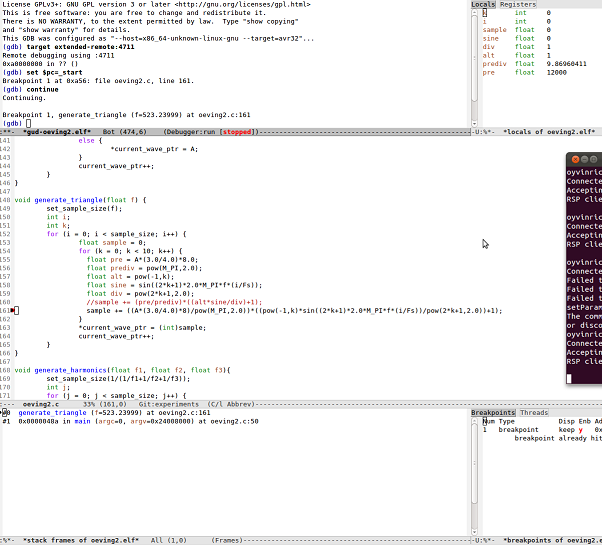
\includegraphics[scale=1]{images/debugsmall.png}
\end{center}

\section{Results}
The result of the exercise is that we coded a single program in C which generates and plays four different sounds when different switches (\emph{SW7} to \emph{SW4}) are pressed. At the start of the program it generates tones (\emph{A4} to \emph{C7}) based on the sine and triangle waves. Then once it gets an interrupt from a switch it plays the first sample of that switch whereafter the ABDAC generates an interrupt which plays the next sample until it is finished.

\section{Tests}
\paragraph{Description}
We've created a few test scenarios in order to test different aspects and corner cases of our code. The main equipment were the STK1000 development board, JTAGICE MKII and a headset.

The setup of the board: 
The headset was connected to the minijack on the development board, the jumper 4 and 5 was set to ''INT. DAC''.
Switches were connected to port C on the parallel I/O, and LED's on port B. 
Both the STK1000 and JTAGICE MKII debugger were connected and powered on. The tests were conducted by a person interacting with the switches wearing a headset, and another person logging the results.

\paragraph{Results}
Below is a table of the different tests we ran, the preconditions and the results. We did not pass the \emph{Bouncing} test. Here we checked whether a sound would play without any interruptions during a switch press (both up and down). 

\begin{center}
\renewcommand{\arraystretch}{1.1} %vertical cell padding
\begin{tabular}[pos]{|m{45pt}|m{80pt}|m{90pt}|m{105pt}|m{60pt}|}
\hline  \textbf{Name} & \textbf{Description} & \textbf{Conditions} & \textbf{Expected} & \textbf{Results} \\ 

\hline Steady-state test & Power is on and the main program is running & The board has been programmed and powered on & The board is powered and no LEDs or sounds should be on & Passed \\

\hline SFX1 & The first SFX plays & The main program is running & \emph{SFX1} plays once after \emph{SW7} is pressed. \emph{LED7} should be turned on & Passed \\

\hline SFX2 & The first SFX plays & The main program is running & \emph{SFX2} plays once after \emph{SW6} is pressed. \emph{LED6} should be turned on & Passed \\

\hline SFX3 & The first SFX plays & The main program is running & \emph{SFX3} plays once after \emph{SW5} is pressed. \emph{LED5} should be turned on & Passed \\ 

\hline Intro theme & The intro theme plays & The main program is running & The intro theme plays once after \emph{SW4} is pressed. \emph{LED4} should be turned on & Passed \\

\hline Bouncing & Any sound should only be played once per press of switch & Press down any switch from \emph{SW7} to \emph{SW4} and let it go & The sound should finish playing without any interruptions & Failed. The sounds is interrupted before finishing. \\

\hline Song change & Play a sound while another sound is already playing & A switch has been pressed and a sound is playing. While playing another switch has been pressed. & The sound of the newly pressed switched should be playing & Passed. \\ 

\hline Stop & Stop playing sounds when pressing any switch from \emph{SW3} to \emph{SW0} & Press any switch from \emph{SW3} to \emph{SW0} while sound is playing & The sound should stop playing & Passed \\ 

\hline 
\end{tabular} 
\end{center}

\section{Evaluation of assignment}
This assignment was more demanding yet also more fun than the first assignment. The learning curve was a bit harder as not all of us had coded much in C before, but it was a nice opportunity to learn.

\section{Conclusion}
We learned how to generate and play different sounds in C. This will be helpful when we start coding the next assignment. In the end we have four different sounds. Three short sound effects and one melody. 

\footnotesize{  % This makes the Reference items print in footnotesize fonts
\begin{thebibliography}{N}

\bibitem[1]{avrdoc} AVR32 Architecture Document
\url{http://www.atmel.com/images/doc32000.pdf}

\bibitem[2]{stkdoc} AT32AP7000 Datasheet
\url{http://www.atmel.com/Images/doc32003.pdf}

\bibitem[3]{komp} TDT4258 Compendium
\url{http://www.idi.ntnu.no/emner/tdt4258/_media/kompendium.pdf}

\end{thebibliography}  
}

\end{document} 
